\documentclass[tikz,border=2cm]{standalone}
\usetikzlibrary {arrows.meta}
\begin{document}
    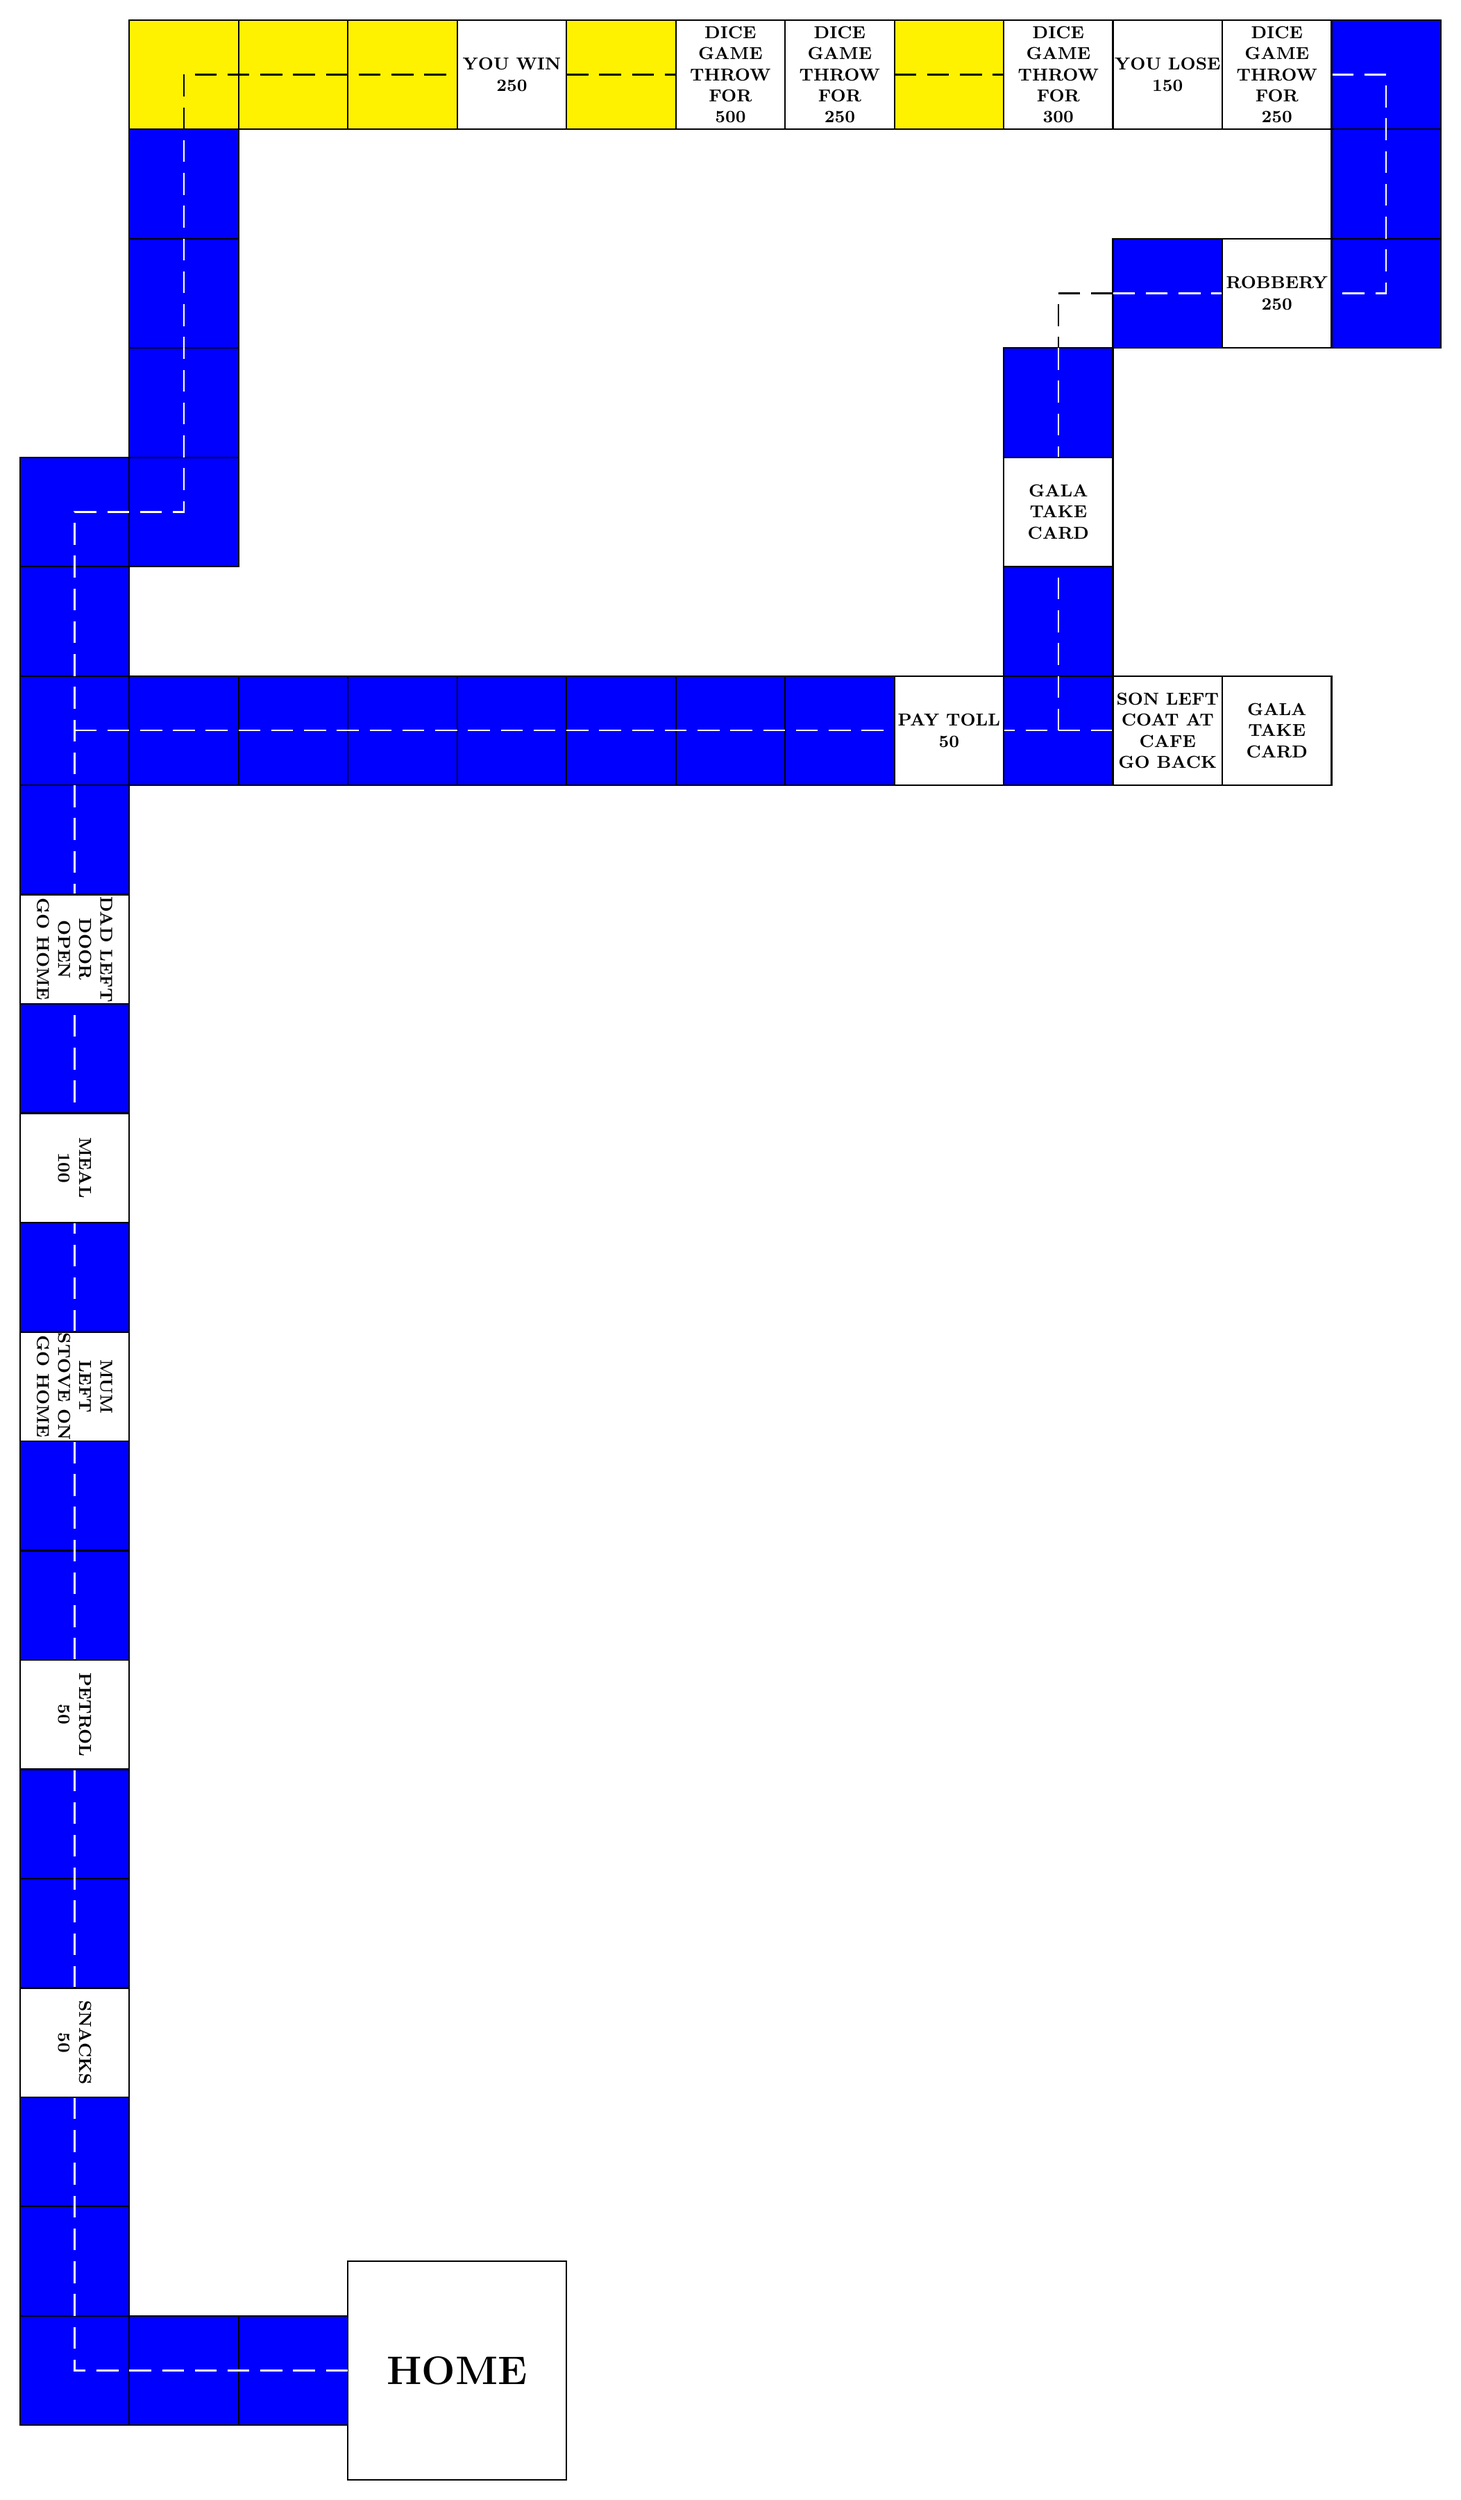
\begin{tikzpicture}
        [every node/.style={rectangle,draw=black,thick,inner sep=0pt,align=center},
        home-square/.style={minimum size=4cm,text width=4cm,font=\huge\bfseries},
        blue-square/.style={fill=blue,minimum size=2cm},
        yellow-square/.style={fill=yellow,minimum size=2cm},
        white-square/.style={minimum size=2cm,text width=2cm,font=\small\bfseries},
        whiteroad/.style={dash pattern=on 4mm off 2mm,thick,white},
        blackroad/.style={dash pattern=on 4mm off 2mm,thick}
        ]
        \node[home-square] (node-0) at (0, 0) {HOME};
        \node[blue-square] (node-1) at (-3, 0) {};
        \node[blue-square] (node-2) at (-5, 0) {};
        \node[blue-square] (node-3) at (-7, 0) {};
        \node[blue-square] (node-4) at (-7, 2) {};
        \node[blue-square] (node-5) at (-7, 4) {};
        \node[blue-square] (node-7) at (-7, 8) {};
        \node[blue-square] (node-8) at (-7, 10) {};
        \node[blue-square] (node-10) at (-7, 14) {};
        \node[blue-square] (node-11) at (-7, 16) {};
        \node[blue-square] (node-13) at (-7, 20) {};
        \node[blue-square] (node-15) at (-7, 24) {};
        \node[blue-square] (node-17) at (-7, 28) {};
        \node[blue-square] (node-18) at (-7, 30) {};
        \node[blue-square] (node-19) at (-7, 32) {};
        \node[blue-square] (node-20) at (-7, 34) {};
        \node[blue-square] (node-21) at (-5, 34) {};
        \node[blue-square] (node-22) at (-5, 36) {};
        \node[blue-square] (node-23) at (-5, 38) {};
        \node[blue-square] (node-24) at (-5, 40) {};
        \node[yellow-square] (node-25) at (-5, 42) {};
        \node[yellow-square] (node-26) at (-3, 42) {};
        \node[yellow-square] (node-27) at (-1, 42) {};
        \node[yellow-square] (node-29) at (3, 42) {};
        \node[yellow-square] (node-32) at (9, 42) {};
        \node[blue-square] (node-36) at (17, 42) {};
        \node[blue-square] (node-37) at (17, 40) {};
        \node[blue-square] (node-38) at (17, 38) {};
        \node[blue-square] (node-40) at (13, 38) {};
        \node[blue-square] (node-41) at (11, 36) {};
        \node[blue-square] (node-43) at (11, 32) {};
        \node[blue-square] (node-44) at (-5, 30) {};
        \node[blue-square] (node-45) at (-3, 30) {};
        \node[blue-square] (node-46) at (-1, 30) {};
        \node[blue-square] (node-47) at (1, 30) {};
        \node[blue-square] (node-48) at (3, 30) {};
        \node[blue-square] (node-49) at (5, 30) {};
        \node[blue-square] (node-50) at (7, 30) {};
        \node[blue-square] (node-52) at (11, 30) {};
        \draw[whiteroad] (-2, 0) -- (-7, 0) -- (-7, 34) -- (-5, 34) -- (-5, 41);
        \draw[blackroad] (-5, 41) -- (-5, 42) -- (0, 42);
        \draw[blackroad] (2, 42) -- (4, 42);
        \draw[blackroad] (8, 42) -- (10, 42);
        \draw[whiteroad] (16, 42) -- (17, 42) -- (17, 38) -- (12, 38);
        \draw[blackroad] (12, 38) -- (11, 38) -- (11, 37);
        \draw[whiteroad] (11, 37) -- (11, 30);
        \draw[whiteroad] (-7, 30) -- (16, 30);
        \node[white-square,rotate=270] (node-6) at (-7, 6) {SNACKS\\50};
        \node[white-square,rotate=270] (node-9) at (-7, 12) {PETROL\\50};
        \node[white-square,rotate=270] (node-12) at (-7, 18) {MUM LEFT\\STOVE ON\\GO HOME};
        \node[white-square,rotate=270] (node-14) at (-7, 22) {MEAL\\100};
        \node[white-square,rotate=270] (node-16) at (-7, 26) {DAD LEFT\\DOOR OPEN\\GO HOME};
        \node[white-square] (node-28) at (1, 42) {YOU WIN\\250};
        \node[white-square] (node-30) at (5, 42) {DICE GAME\\THROW FOR\\500};
        \node[white-square] (node-31) at (7, 42) {DICE GAME\\THROW FOR\\250};
        \node[white-square] (node-33) at (11, 42) {DICE GAME\\THROW FOR\\300};
        \node[white-square] (node-34) at (13, 42) {YOU LOSE\\150};
        \node[white-square] (node-35) at (15, 42) {DICE GAME\\THROW FOR\\250};
        \node[white-square] (node-39) at (15, 38) {ROBBERY\\250};
        \node[white-square] (node-42) at (11, 34) {GALA\\TAKE\\CARD};
        \node[white-square] (node-51) at (9, 30) {PAY TOLL\\50};
        \node[white-square] (node-53) at (13, 30) {SON LEFT\\COAT AT\\CAFE\\GO BACK};
        \node[white-square] (node-54) at (15, 30) {GALA\\TAKE\\CARD};
    \end{tikzpicture}
\end{document}